\section{R\'esultats et visualisations}
\label{sec:resultats}

L'\'evaluation a \'et\'e ex\'ecut\'ee sur les 34 questions du jeu de test. Le
tableau~\ref{tab:metrics} r\'esume les moyennes obtenues.

\begin{table}[H]
  \centering
  \caption{Moyennes des m\'etriques d'\'evaluation (34 questions).}
  \label{tab:metrics}
  \begin{tabular}{@{}lc@{}}
    \toprule
    \textbf{M\'etrique} & \textbf{Valeur moyenne} \\
    \midrule
    Precision@3 & 0.922 \\
    Recall@3 & 0.985 \\
    Fid\'elit\'e (faithfulness) & 0.887 \\
    Temps de r\'eponse (s) & 0.811 \\
    \bottomrule
  \end{tabular}
\end{table}

\subsection{Synth\`ese des m\'etriques}

La figure~\ref{fig:avg} pr\'esente les moyennes des trois scores principaux (precision, recall,
fid\'elit\'e). Le recall moyen tr\`es \'elev\'e (0.985) indique que le retriever retrouve
quasi syst\'ematiquement au moins un chunk du document attendu. La precision l\'eg\`erement
inf\'erieure (0.922) refl\`ete des cas o\`u un ou deux des trois chunks proviennent de documents
voisins s\'emantiquement proches (voir section~\ref{sec:discussion}).

\begin{figure}[H]
  \centering
  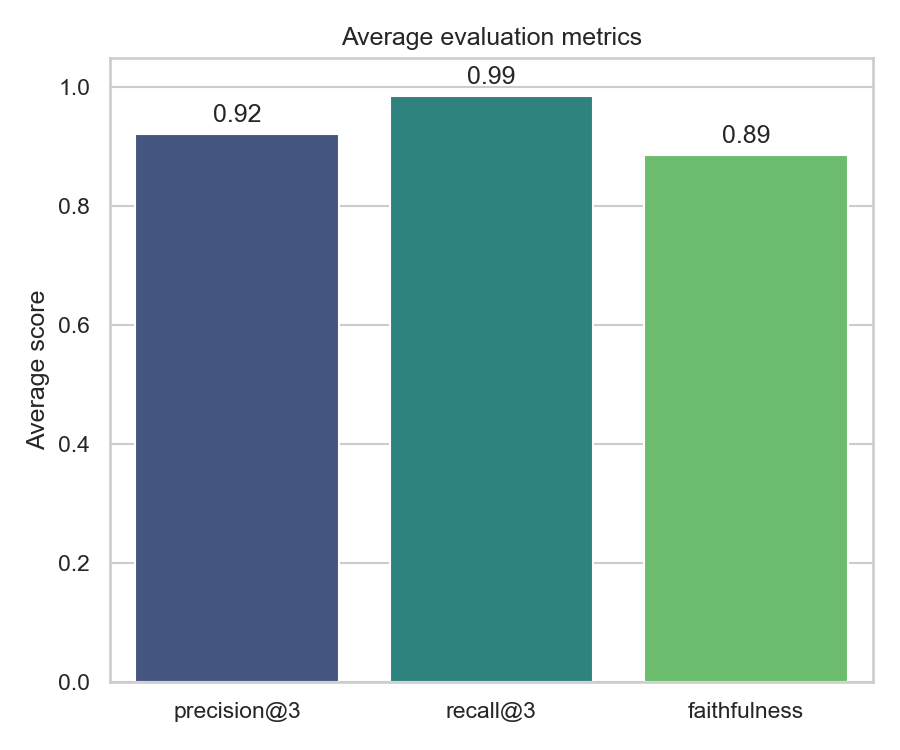
\includegraphics[width=0.62\textwidth]{figures/average_metrics.png}
  \caption{Moyennes des m\'etriques d'\'evaluation sur les 34 questions.}
  \label{fig:avg}
\end{figure}

\subsection{Precision et recall par question}

La figure~\ref{fig:pr} d\'etaille Precision@3 et Recall@3 pour chaque question. La majorit\'e
des questions atteignent un score de 1.0 ; quelques exceptions correspondent \`a des sujets
proches (FastText / Word2vec, lemmatisation / stemmatisation, etc.).

\begin{figure}[H]
  \centering
  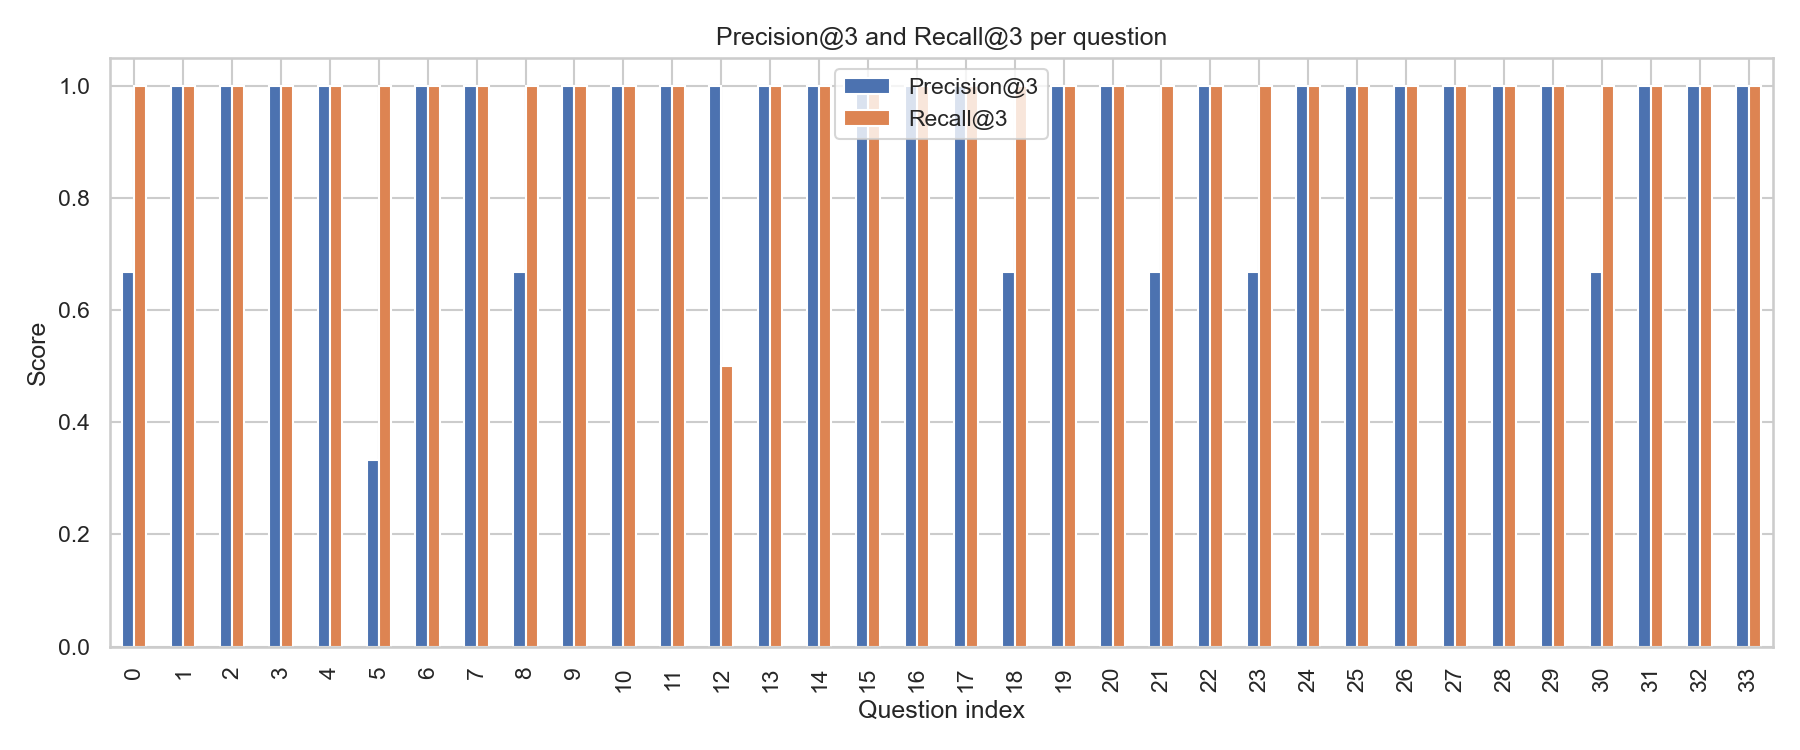
\includegraphics[width=\textwidth]{figures/precision_recall_per_question.png}
  \caption{Precision@3 et Recall@3 pour chacune des 34 questions.}
  \label{fig:pr}
\end{figure}

\subsection{Distribution de la fid\'elit\'e}

La figure~\ref{fig:faith} montre la distribution du score de fid\'elit\'e lexicale. La plupart
des r\'eponses d\'epassent 0.8, ce qui indique un bon ancrage dans le contexte r\'ecup\'er\'e.
Quelques scores plus bas (par exemple pour la question sur BERT, fid\'elit\'e = 0.484) s'expliquent
par des reformulations correctes utilisant un vocabulaire diff\'erent de celui des chunks, limite
connue de la m\'etrique lexicale.

\begin{figure}[H]
  \centering
  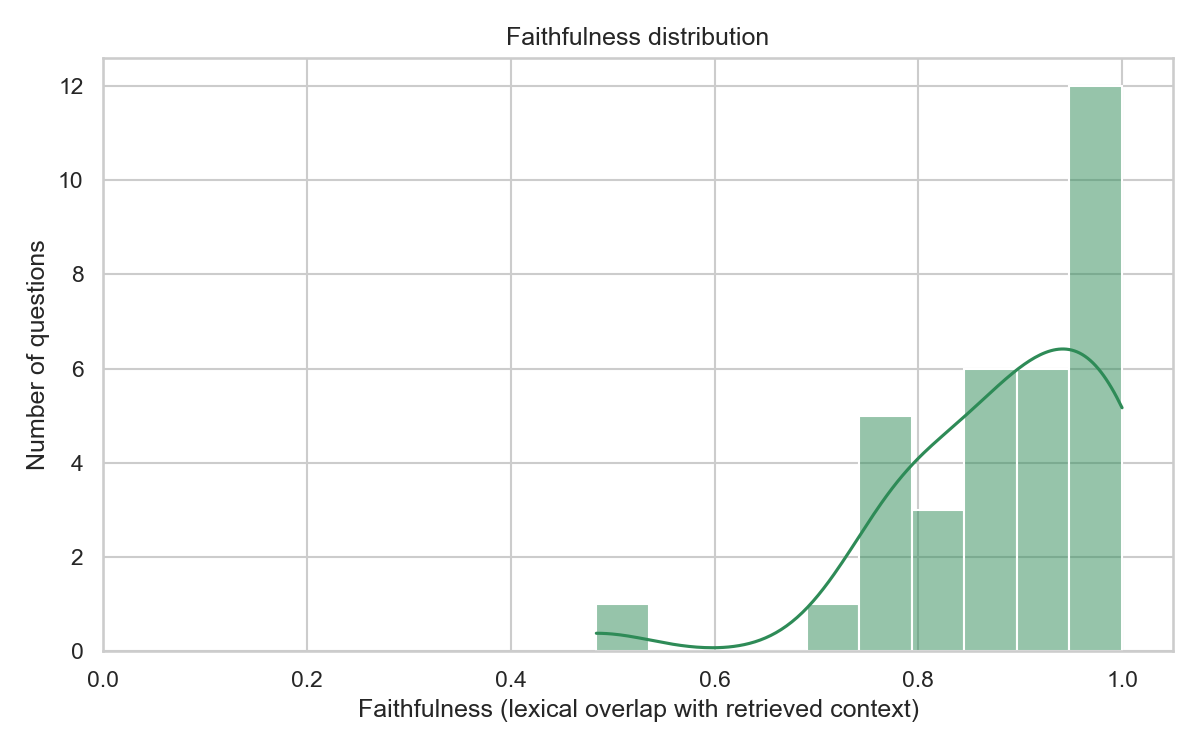
\includegraphics[width=0.72\textwidth]{figures/faithfulness_distribution.png}
  \caption{Distribution du score de fid\'elit\'e (recouvrement lexical avec le contexte).}
  \label{fig:faith}
\end{figure}

\subsection{Temps de r\'eponse}

La figure~\ref{fig:time} pr\'esente la distribution des temps de r\'eponse. La majorit\'e des
questions sont trait\'ees en moins d'une seconde ; quelques valeurs plus \'elev\'ees (jusqu'\`a
3.5~s) correspondent \`a des r\'eponses plus longues ou \`a une latence r\'eseau ponctuelle de
l'API Groq.

\begin{figure}[H]
  \centering
  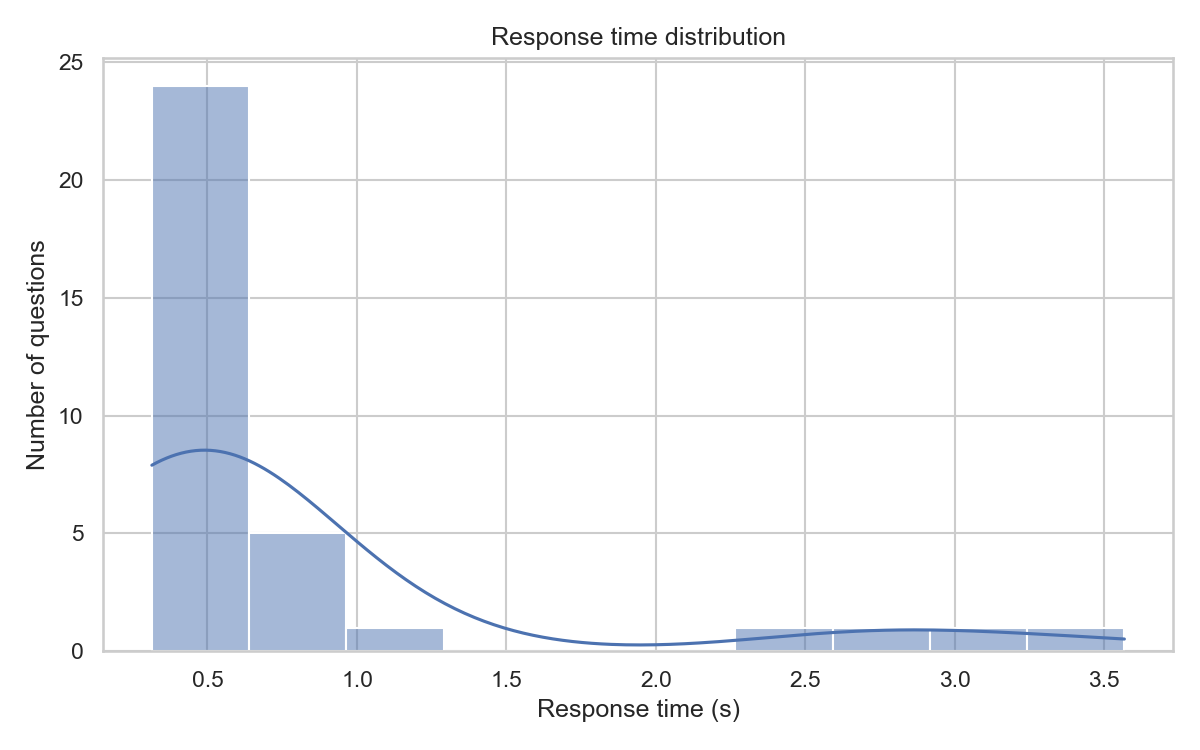
\includegraphics[width=0.72\textwidth]{figures/response_time_distribution.png}
  \caption{Distribution des temps de r\'eponse (secondes).}
  \label{fig:time}
\end{figure}

\subsection{Relation temps / fid\'elit\'e}

La figure~\ref{fig:scatter} croise temps de r\'eponse, fid\'elit\'e et precision@3. Aucune
corr\'elation forte n'appara\^it : une r\'eponse plus lente n'est ni syst\'ematiquement plus
fid\`ele, ni moins pr\'ecise.

\begin{figure}[H]
  \centering
  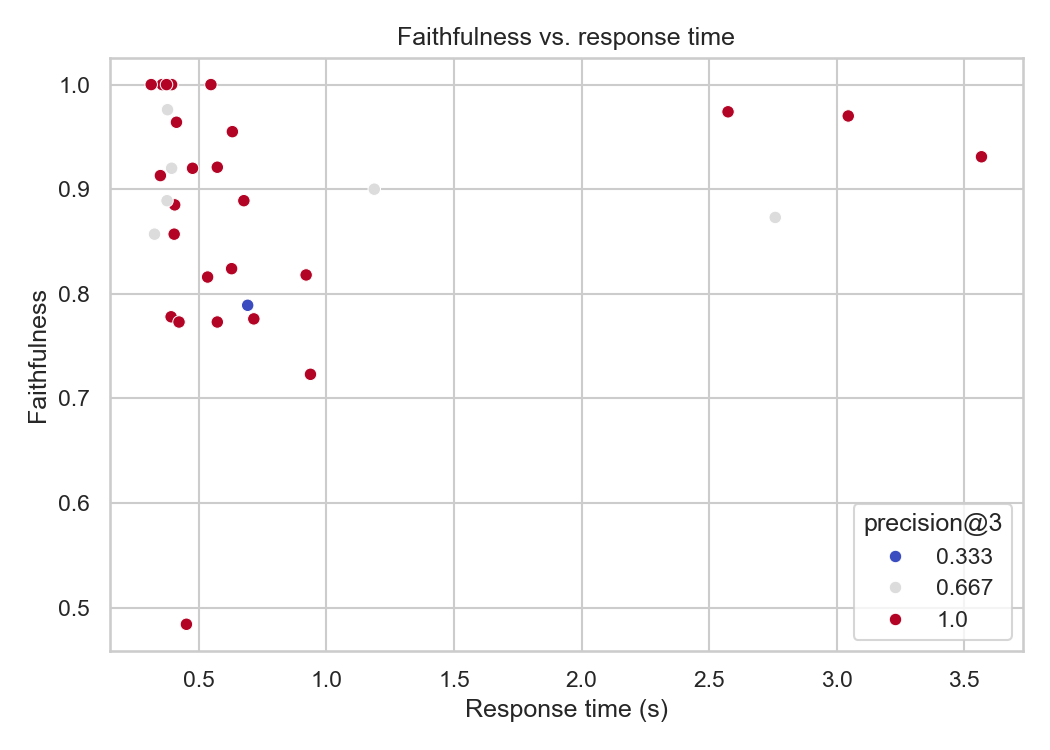
\includegraphics[width=0.72\textwidth]{figures/time_vs_faithfulness.png}
  \caption{Temps de r\'eponse, fid\'elit\'e et precision@3 (couleur).}
  \label{fig:scatter}
\end{figure}

\subsection{Questions \`a scores plus faibles (extrait)}

\begin{table}[H]
  \centering
  \caption{Exemples de questions avec precision@3 inf\'erieure \`a 1.0.}
  \label{tab:lowprec}
  \small
  \begin{tabular}{@{}p{5.8cm}cc@{}}
    \toprule
    \textbf{Question (abr\'eg\'ee)} & \textbf{Prec.@3} & \textbf{Recall@3} \\
    \midrule
    FastText vs earlier embeddings & 0.333 & 1.0 \\
    Attention mechanism in ML & 0.667 & 1.0 \\
    GloVe word vectors training & 0.667 & 1.0 \\
    Lemmatization vs stemming & 1.0 & 0.5 \\
    Sentence embedding uses & 0.667 & 1.0 \\
    \bottomrule
  \end{tabular}
\end{table}

Ces cas illustrent la difficult\'e d'attribuer un unique document ``gold'' lorsque plusieurs
articles du corpus traitent de notions voisines.
